\section{Experiments}
Many experiment runs were conducted using different benchmarks to understand how the dispatch bandwidth (n) and scheduling queue size (s) affects the performance of the scheduler. The following sections explains the experiment runs, the scheduler configuration and the results in tables and graphs for two different benchmarks --- gcc and perl.


\subsection{Benchmark gcc}
In this experiment the scheduler is run with different possible configurations (varying values of \textit{n} and \textit{s}) against the gcc benchmark. The dispatch bandwidth is varied in powers of 2 from 1 till 8 and the scheduling queue size is varied from 8 till 256, in powers of 2 again. For each such configuration, the IPC is calculated. The results are tabulated in table \ref{tab:gcc} and the results are plotted as line curves for \textit{s} vs \textit{IPC} for different values of \textit{n} in figure \ref{fig:gcc}.

\begin{table}[htbp]
    \centering
    \noindent \begin{tabular}{|c|c|c|c|c|}
        \hline
        \multirow{2}[4]{*}{\bf Scheduling Queue Size (s) } & \multicolumn{4}{c|}{\bf Instructions Per Cycle (IPC)} \\
        \cline{2-5} & \bf n = 1 & \bf n = 2 & n = 4 & \bf n = 8 \\
        \hline
          8 & 0.99 & 1.88 & 2.67 & 2.82 \\
         16 & 1.00 & 1.99 & 3.54 & 4.54 \\
         32 & 1.00 & 1.99 & 3.90 & 6.48 \\
         64 & 1.00 & 1.99 & 3.97 & 7.52 \\
        128 & 1.00 & 1.99 & 3.97 & 7.83 \\
        256 & 1.00 & 1.99 & 3.97 & 7.83 \\
        512 & 1.00 & 1.99 & 3.97 & 7.83 \\
        \hline
    \end{tabular}
    \captionsetup{justification=centering}
    \caption{Dynamic Scheduler Experiment Data for gcc Benchmark for different \textit{n} and \textit{s} values}
    \label{tab:gcc}
\end{table}

\begin{figure} [htbp]
    \centering
    \noindent {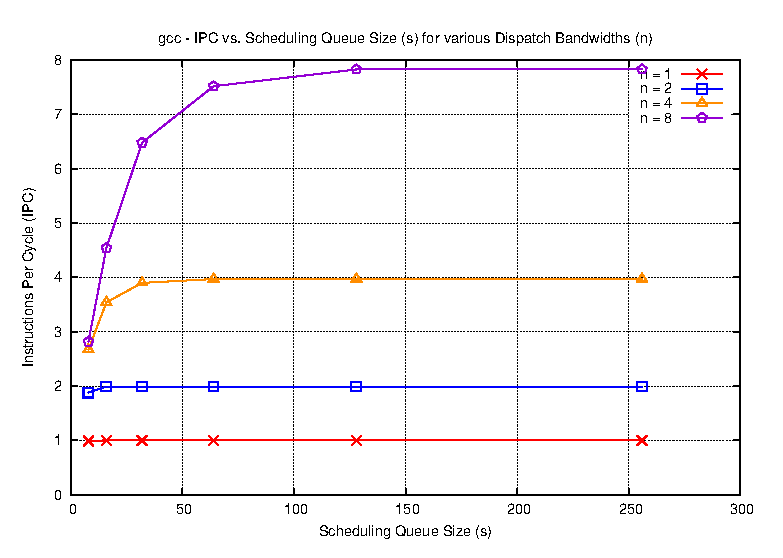
\includegraphics[width=\textwidth, keepaspectratio]{img/gcc.eps}}
    \caption{Scheduling Queue Size vs Instructions Per Cycle for gcc Benchmark}
    \label{fig:gcc}
\end{figure}


\subsection{Benchmark perl}
In this experiment the scheduler is run with different possible configurations (varying values of \textit{n} and \textit{s}) against the perl benchmark. The dispatch bandwidth is varied in powers of 2 from 1 till 8 and the scheduling queue size is varied from 8 till 256, in powers of 2 again. For each such configuration, the IPC is calculated. The results are tabulated in table \ref{tab:perl} and the results are plotted as line curves for \textit{s} vs \textit{IPC} for different values of \textit{n} in figure \ref{fig:perl}.

\begin{table}[htbp]
    \centering
    \noindent \begin{tabular}{|c|c|c|c|c|}
        \hline
        \multirow{2}[4]{*}{\bf Scheduling Queue Size (s) } & \multicolumn{4}{c|}{\bf Instructions Per Cycle (IPC)} \\
        \cline{2-5} & \bf n = 1 & \bf n = 2 & n = 4 & \bf n = 8 \\
        \hline
          8 & 0.98 & 1.68 & 2.18 & 2.28 \\
         16 & 1.00 & 1.89 & 2.91 & 3.37 \\
         32 & 1.00 & 1.98 & 3.68 & 5.18 \\
         64 & 1.00 & 1.98 & 3.91 & 6.95 \\
        128 & 1.00 & 1.98 & 3.94 & 7.61 \\
        256 & 1.00 & 1.98 & 3.94 & 7.75 \\
        512 & 1.00 & 1.98 & 3.94 & 7.75 \\
        \hline
    \end{tabular}
    \captionsetup{justification=centering}
    \caption{Dynamic Scheduler Experiment Data for for perl Benchmark for different \textit{n} and \textit{s} values}
    \label{tab:perl}
\end{table}

\begin{figure} [htbp]
    \centering
    \noindent {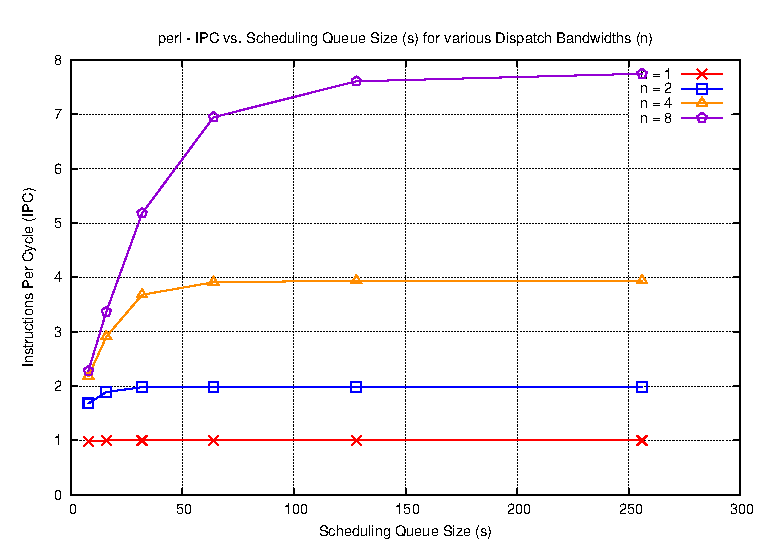
\includegraphics[width=\textwidth, keepaspectratio]{img/perl.eps}}
    \caption{Scheduling Queue Size vs Instructions Per Cycle for perl Benchmark}
    \label{fig:perl}
\end{figure}
